\documentclass[10pt,a4paper]{article}
\usepackage[utf8]{inputenc}
\usepackage{amsmath}
\usepackage{amsfonts}
\usepackage{tikz}
\usetikzlibrary{shapes,arrows,automata,fit}
\usepackage{amssymb}
\usepackage{graphicx}
\usepackage{wrapfig}
\usepackage{helvet}
\usepackage{pgf-umlsd}
\usepackage{textcomp}
\author{Gokudomatic}
\title{Documentation of the Fox2d demo project}
\date{\today\\v1.1}
\renewcommand{\familydefault}{\sfdefault}

\tikzstyle{node} = [draw, fill=blue!20, text centered, rounded corners]
\tikzstyle{decision} = [diamond, draw, fill=blue!20, 
    text width=4.5em, text badly centered, node distance=3cm, inner sep=0pt]
\tikzstyle{block} = [rectangle, draw, fill=blue!20, 
    text width=5em, text centered, rounded corners, minimum height=4em]
\tikzstyle{line} = [draw, -latex']
\tikzstyle{cloud} = [draw, ellipse,fill=red!20, node distance=3cm,
    minimum height=2em]

\tikzset{
  line/.style ={draw, thick, -latex', shorten >=0pt}
}

\begin{document}

\maketitle

\clearpage

\begin{center}
{\Large Revisions}
\begin{tabbing}
\hspace{1cm} \= \kill
1.0 \> Original version using Kirby's assets\\
1.1 \> All visual assets and musics from Kirby are replaced by free to use assets
\end{tabbing}
\end{center}

\clearpage

\tableofcontents

\clearpage

\section{Introduction}

\subsection{Purpose}
The purpose of this document is to explain how the demo project Fox2d is done. This project is a demo made with the Game Engine Godot\cite{godot}, and it have been made in the context of learning 2d platform games with Godot, and it has been commented and document so it can help new people to start with Godot. \\
It is however important to note that \textbf{it's a documented demo and not a tutorial}. It won't explain the procedure step by step how to make the demo.

\subsection{Target audience}
This document is destined to those who begin with Godot Engine. A basic knowledge of the Godot IDE and GDScript is still required, as well as some knowledge in general programming.

\subsection{Where to start}
As said, this document is not a tutorial. The best approach is to get familiarized first with the demo by playing with it. Then, with both Godot and this document opened, discover how are made the main actors, the singleton script files, and the levels.

\subsection{About Godot Engine}
\paragraph{}
The Godot Engine is a game engine with its own visual editor and script language. This engine and tool have been internally developed since 2001 by Okame for its own games. Since February 2014 it became open source with MIT licence and it's free to use. Not only it supports compilation for many platforms, as Android, Windows, Linux, Mac, etc., but the editor itself supports also multiple platforms, namely Windows, Linux and Mac.
\paragraph{Highlights of the engine}
Unlike most of others existing game engines and game authoring tools, Godot Engine offers both a visual editor and a scripting language. The user don't have then to program the whole game at hand in source code, like it would be for most game engines, and yet it doesn't sacrifice the flexibility of scripting in sake of "making it affordable for non developers" like most game makers do. 
\paragraph{Nodes}
The game engine is composed with nodes. Everything is a node, except for standard libraries for scripting and stuff from the engine itself (script engine, display, input, etc.). However everything that is visible is a node. \\
A node is an object that has properties, functions and a custom script. Like in a XML tree, a node has a parent and can have children, all of them being nodes too. Nodes are the fundamental bricks of the game. And they have also the capability to inherit from others nodes the same way as in object oriented programming. Some of them are native nodes coded in C++, and others are extending from the native ones.
\paragraph{Scenes}
The scene is a special node that be edited by the visual editor of Godot. A scene in Godot represents either literally a scene, where objects are shown and animated, either an actor of the game. The scene is a native node, yet it's not specific which node it must be. Usually a Node (the most abstract and common native node type) or a Node2D/Spatial (abstract node with spatial reference) is used as the node of a scene. And under this node are added others nodes like sprites and physic bodies, but it can be any kind of node, even a music player.
What make scenes particular is that they can be used like objects in others scenes. Typically a sprite that moves and get animated would be a scene on its own and it would be added to another scene that represents the level of the game, with a terrain, monsters and others stuffs. And with scripting, the scene can be extended in its functionalities. That makes the scene one of the most versatile nodes of the engine, and the most used one by the user to create his game assets.
\paragraph{GDScript}
GDscript is a custom scripting language based on Python syntax. The language is very simple and can be learned in one day. It suffers however from being young and with only a small framework. Its selling point however is its deep integration with the node system and internal threads of the engine. It results in a very efficient and pragmatical language that gives good performances even on platforms with limited resources.\\
And this gives also the feature to chose how to structure the code. The script can be contained in a class file, or directly embedded in a scene, or even directly embedded in an instance of a scene. Having those three possibilities allows to very simply and efficiently write the code without having the framework in the way. The drawback, however, is the risk of inconsistency in the project and hard maintainability. It is very recommended, when starting a medium to large project, to set strict rules about code architecture. And breaking the rules should be avoided as much as possible but still allowed to make some tweaks that would very hard to implement otherwise.

\subsection{About the author}
I'm essentially a programmer with a few experience in 2d and 3d graphics. I have some personal experience in game programming, mostly in Java and Delphi, yet all my projects were for personal training and didn't reach any public status.

\section{Game}

\subsection{In a nutshell}
This demo is based on the popular Nintendo's\cite{nintendo} franchise Kirby\cite{kirby} (Figure \ref{fig:original_game}). It started in the nineties on Gameboy as a very simple and easy platform game for young kids, and then it evolved way beyond anyone's expectation thanks to the huge potential in its game concept. \\
This demo is based on the very first game, without all the actual mechanics of the franchise. The reason is mostly because it's simple and yet it uses lot of fundamental features of a platform game.

\begin{figure}
\centering
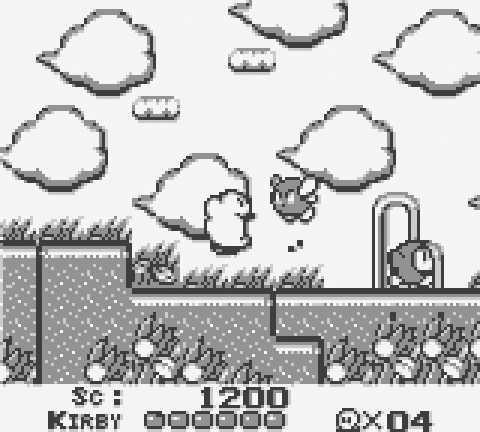
\includegraphics[bb=0 0 480 432,width=6cm]{KDL4.png} 
\caption{Original Kirby game}
\label{fig:original_game}
\end{figure}

\subsection{Gameplay}
The player moves in a 2d linear world, can jump and fall, and has one special power, which is to eat almost anything. This power is however very versatile. The player can create a vacuum in which every enemy and movable object get sucked and eaten. Then the player can "spite" the result his digestion, which happen to be star shaped and that can hurt enemies it touches. The player can also suck air and inflate like a balloon, which gives him the ability to float freely (but slowly). In the second game of the franchise, a new mechanism of absorbing the power of an enemy is introduced, which extends even more the versatility of the player's power.

\section{Project structure}

\subsection{file structure}
In this demo, the files are meant to be structured this way:
\begin{itemize}
 \item audio : all sounds and musics.
 \item res : all graphics.
 \item enemies : common assets for enemies.
 \item maps : levels of the game and their specific scripts.
\end{itemize}
Actually most assets and files were thrown at the root folder because of convenience. But when the project gets bigger, it will be needed to restructure files in a more meaningful folder structure. \\
Important files are:
\begin{itemize}
 \item engine.cfg : the project definition file.
 \item main.scn : the very first scene automatically loaded. It acts like a scene loader and manages the HUD (heads-up display).
 \item global.gd : singleton utility script for scene loading and playing music.
 \item soundmanager.res : singleton node managing background musics and sounds that are meant to be played through scenes without interruption.
 \item game\_data.gd : singleton script that manages game's common data, like player's life and high score.
\end{itemize}
\subsection{Node structure}
Figure \ref{fig:node_struct} is the general structure of nodes running in the game.
It is composed by singletons and layers. \\
\textbf{Singletons} are classes that provide data and functions through levels. They are not visible. \\
\textbf{MapLayer} is in fact not a layer but a Node for technical reasons. However it acts like a layer which contains the scene of the current level or cut-scene. Therefore its children are regularly removed and replaced by new ones. But the node itself is never removed or modified. \\
\textbf{HudLayer} contains common visual nodes that come in every level, like player's life bar, high score, etc. \\
\textbf{ScreenEffectLayer} is a node that can make the whole screen white by playing with its transparency. It is used for scene transition.

\begin{figure}[h]
\centering
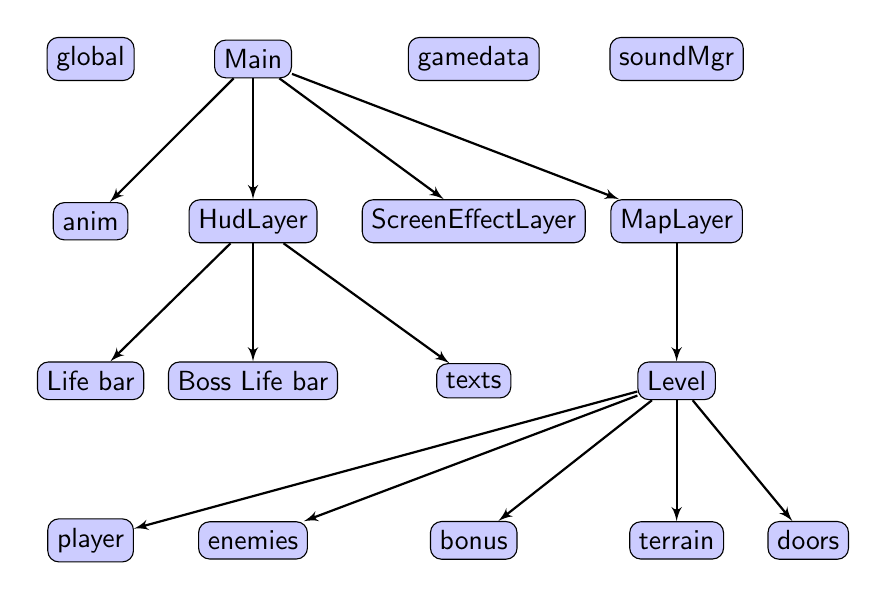
\begin{tikzpicture}
 \matrix [column sep=3mm, row sep=15mm] {
    \node[node] (global) {global}; 
   & \node[node] (root) {Main}; 
   & \node[node] (game_data) {gamedata}; 
   & \node[node] (soundmgr) {soundMgr}; \\
    \node[node] (anim) {anim};  
   & \node[node] (hud) {HudLayer};
   & \node[node] (screeneffect) {ScreenEffectLayer};  
   & \node[node] (map) {MapLayer}; \\
   
   \node[node] (lifebar) {Life bar}; 
   & \node[node] (bosslifebar) {Boss Life bar}; 
   & \node[node] (hudtext) {texts}; 
   & \node[node] (level) {Level}; \\
   \node[node] (player) {player};
   & \node[node] (enemies) {enemies};
   & \node[node] (bonus) {bonus};
   & \node[node] (terrain) {terrain};
   & \node[node] (doors) {doors}; \\
 };
 \begin{scope}[every path/.style=line]
   \path (root) -- (map);
   \path (root) -- (hud);
   \path (root) -- (screeneffect);
   \path (root) -- (anim);
   \path (map) -- (level);
   \path (hud) -- (lifebar);
   \path (hud) -- (bosslifebar);
   \path (hud) -- (hudtext);
   \path (level) -- (player);
   \path (level) -- (enemies);
   \path (level) -- (bonus);
   \path (level) -- (terrain);
   \path (level) -- (doors);

 \end{scope}
 
\end{tikzpicture}
\caption{General structure of nodes}
\label{fig:node_struct}
\end{figure}

\clearpage

\section{Actors}

\subsection{Player}
\begin{wrapfigure}{L}{0.1\textwidth}

\includegraphics[bb=0 0 48 48,scale=0.5]{kirby.png} 
\end{wrapfigure}
The player is the only playable actor of this demo. It has a state, follow rules of a state machine.
\paragraph{Node structure}
The root of the player is a KinematicBody2D.
It is composed of: \\
\begin{tabular}{ l  l }
  \textit{Sprite} & The image of the actor \\
  \textit{collisionShape} & hitbox of the player for physics collisions, used by the root node \\
  \textit{anim} & Animation player of the actor, mostly for the sprite \\
  \textit{Camera2D} & The camera following the actor \\
  \textit{breath\_shoot} & Point for spawning a bullet\\
  \textit{cone\_shoot} & Point for spawning the vacuum cone\\
  \textit{Area2D} & Hitbox of the player for enemies and bonus \\
  \textit{enemyActivator} & Area for activating enemies\\
  \textit{traverseTimer} & Timer for traversing floors\\
  \textit{sfx} & Sound manager for the player\\
\end{tabular}
\paragraph{State machine}
The player has multiple states, as in Figure \ref{fig:player_state_machine}. Its initial state is \textit{normal}.\\
When in cutscene mode, the player doesn't listen anymore to inputs nor it gets influenced by physics. The idea is that an animation player takes care of moving the actor.
\begin{figure}[h]
\centering
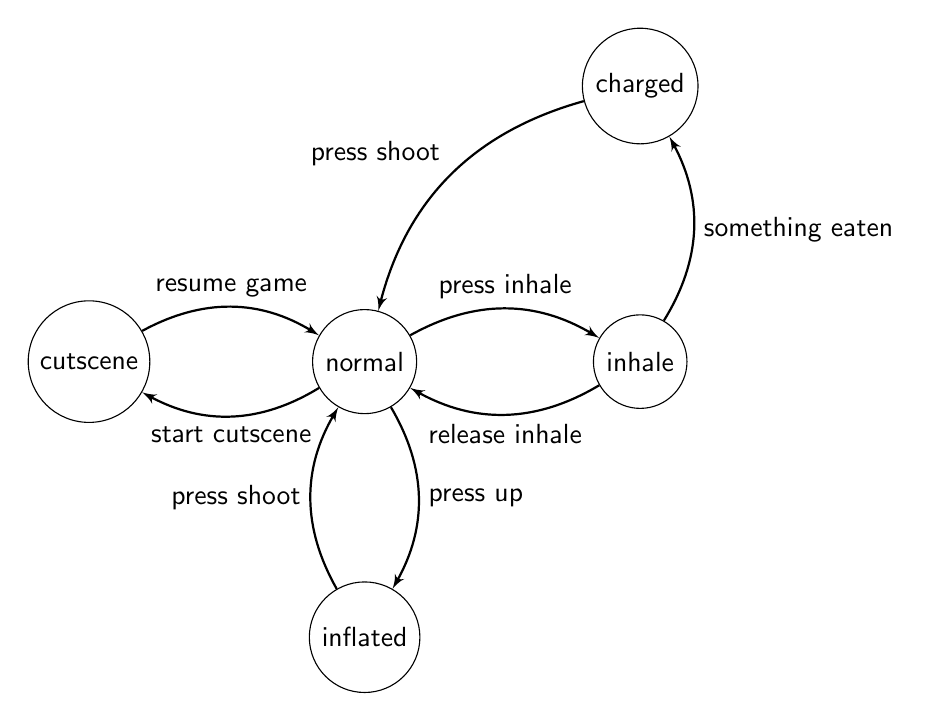
\begin{tikzpicture}[>=stealth',shorten >=1pt,auto,node distance=3.5cm]
  \node[state] (normal) {normal};
  \node[state,right of=normal] (inhale) {inhale};
  \node[state,above of=inhale] (charged) {charged};
  \node[state,below of=normal] (inflated) {inflated};
  \node[state,left of=normal] (cutscene) {cutscene};

  \begin{scope}[every path/.style=line]
    \path[->] (normal) edge [bend left] node[above] {press inhale} (inhale);
    \path[->] (inhale) edge [bend left] node[below] {release inhale} (normal);
    \path[->] (inhale) edge [bend right] node[swap] {something eaten} (charged);
    \path[->] (charged) edge [bend right] node[swap] {press shoot} (normal);
    \path[->] (normal) edge [bend left] node[swap,right] {press up} (inflated);
    \path[->] (inflated) edge [bend left] node[swap,left] {press shoot} (normal);
    \path[->] (normal) edge [bend left] node[swap,below] {start cutscene} (cutscene);
    \path[->] (cutscene) edge [bend left] node[swap,above] {resume game} (normal);
  \end{scope}
  
\end{tikzpicture}
\caption{Player's state machine}
\label{fig:player_state_machine}
\end{figure}

\subsection{Common enemy}
Enemies are very identical. Only their sprite and their movement pattern change. Thus, instead of copying the same node structure into the node of each kind of enemy, one node is used by all enemies, with all sprites, and only their script and a parameter for the sprite change.\\
It has the advantage of being easier to maintain, but the disadvantages of limitations in what the enemy can do and its collision shape (limitation of the engine at the time when this document was written. Maybe a solution will be found in the future).
\paragraph{Node Structure}
The root of the enemy is a KinematicBody2D, implementing the Edible class.
It is composed of: \\
\begin{tabular}{ l  l }
  \textit{sprite} & The image of the actor \\
  \textit{CollisionShape2D} & Hitbox of the actor, used by the root node \\
  \textit{AnimationPlayer} & Animation player of the actor, mostly for the sprite \\
  \textit{animTreePlayer} & Manager of the different animations for all types of enemies \\
  \textit{raycast\_left} & Collision sensor \\
  \textit{raycast\_right} & Collision sensor \\
  \textit{explodeSprite} & Image of the explosion of the actor \\
\end{tabular}

\paragraph{Sensors}
The sensors of the common enemy, which are called Raycast2D in Godot, are a special kind of node that can check if their colliding with something else. Thanks to their position, as in Figure \ref{fig:enemy_sensor}, the enemy can then know if he's about to collide with something and can make a decision, like turn the other way. \\
\textbf{Note} : This feature is not always used, depending on the movement pattern. Some kinds of enemy just don't need it.

\begin{figure}[h]
\centering
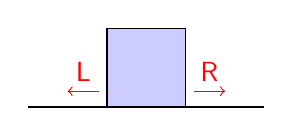
\begin{tikzpicture}
	\draw[fill=blue!20] (0,0) rectangle (1,1);
	\draw (-1,0) -- (2,0);
	\draw[->,draw=red] (-0.1,0.2) -- node[swap,above] {\color{red}L} (-0.5,0.2);
	\draw[->,draw=red] (1.1,0.2) -- node[swap,above] {\color{red}R} (1.5,0.2);
\end{tikzpicture}
\caption{Sensors of the enemy, in red}
\label{fig:enemy_sensor}
\end{figure}

\paragraph{Animation tree}
The sprites are managed by the Animation Tree Player, as in Figure \ref{fig:common_enemy_anim_tree}.
The node \textit{transition} is the one deciding which kind of enemy to display, where the node \textit{Eagle transition} defines more precisely in which state is the enemy for this specific kind.
\begin{figure}
\centering
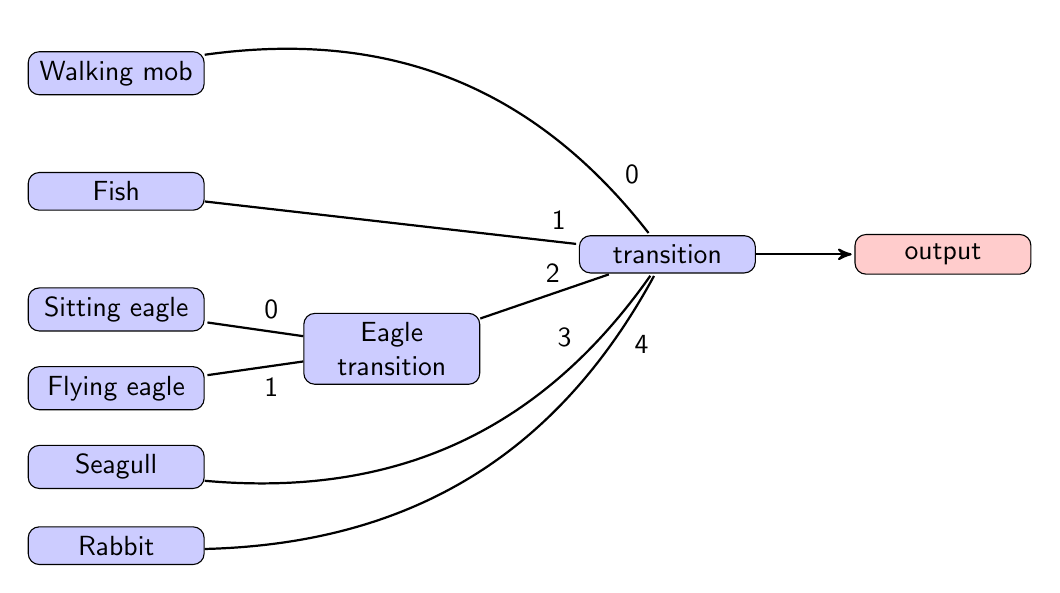
\begin{tikzpicture}[>=stealth',shorten >=1pt,auto,node distance=3.5cm,text width=2cm]
  \node[node] (switcher) {transition};
  \node[node,right of=switcher,fill=red!20] (output) {output};
  \node[node,yshift=-12mm,left of=switcher] (birdTransition) {Eagle transition};
  \node[node,yshift=5mm,left of=birdTransition] (bird1) {Sitting eagle};
  \node[node,yshift=-5mm,left of=birdTransition] (bird2) {Flying eagle};

  \node[node,above of=bird1,node distance=1.5cm] (mushroom1) {Fish};

  \node[node,above of=mushroom1,node distance=1.5cm] (mob) {Walking mob};
  \node[node,below of=bird2,node distance=1cm] (fly) {Seagull};
  \node[node,below of=fly,node distance=1cm] (lutin) {Rabbit};

  \begin{scope}[every path/.style=draw,thick]
    \path[->] (switcher) -- (output);
    \path (mushroom1) -- node[pos=0.9] {1} (switcher);
    \path (birdTransition) -- node[swap,above,pos=1.1,yshift=-3mm] {2} (switcher);
    \path (mob) edge[bend left] node[pos=0.9] {0} (switcher);
    \path (fly) edge[bend right] node[swap,above,pos=0.8,xshift=7mm] {3} (switcher);
    \path (lutin) edge[bend right] node[swap,pos=0.9] {4} (switcher);
    \path (birdTransition) -- node[swap] {0} (bird1);
    \path (birdTransition) -- node {1} (bird2);
  \end{scope}
  
\end{tikzpicture}
\caption{Animation tree of the common enemy}
\label{fig:common_enemy_anim_tree}
\end{figure}

\clearpage

\subsection{Boss}
\begin{wrapfigure}{L}{0.1\textwidth}

\includegraphics[bb=0 0 54 75,scale=0.5]{boss.png} 
\end{wrapfigure}
The boss is a special kind of enemy with the following characteristics:
\begin{itemize}
\item Cannot be eaten.
\item Has multiple patterns.
\item Can throw infinitely mobs or bombs, which the player must use to shoot a star to the boss.
\item Has a life bar.
\item Has its own stage (player cannot leave and camera is fixed).
\end{itemize}

\textit{Note : In version 1.1 bomb's visual asset is replaced by a rock. But its behavior didn't change.}

\paragraph{Node structure}
In the context of this demo, this kind of boss had complex but static movement patterns, where he always go back to its original position. And so the movements are done with an animation player. An attempt was made by creating a sub-node that represents the collidable actor, which might not be the best solution. But it works. This sub-node is moved by the animation player.
Its root is a KinematicBody2D, implementing the Edible class.
It is composed of: \\
\begin{tabular}{ l  l }
  \textit{actor\_boss} & Sub-node containing the sprite and collision shape \\
  \textit{sprite} & The image of the actor \\
  \textit{CollisionShape2D} & Hitbox of the actor, used by the root node \\
  \textit{explosion} & The image of the explosion \\
  \textit{bombSpawnPos} & Position where to spawn a bomb \\
  \textit{anim} & Animation player \\
\end{tabular}

\paragraph{Movement pattern}
Bosses will always be implemented specifically for their needs because they have little in common. One can be just jumping here and there, where another one rushes to the player or go through different transformations. For the boss of this demo, the pattern is like in Figure \ref{fig:boss_state_machine}.
\begin{figure}[h]
\centering
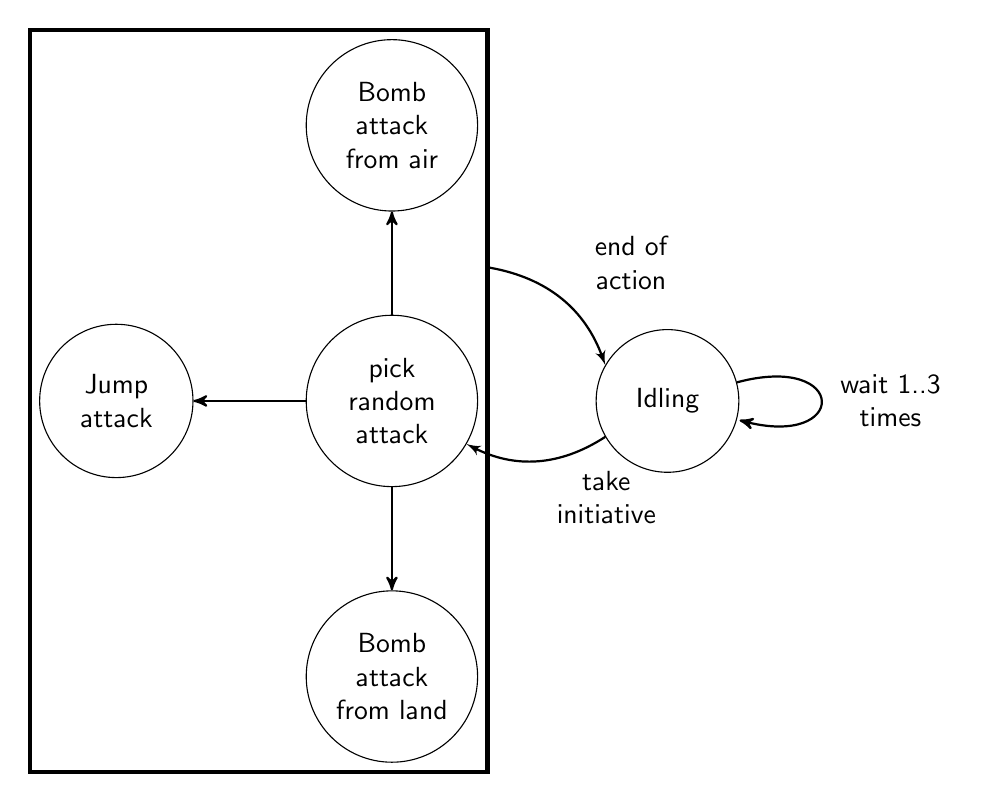
\begin{tikzpicture}[>=stealth',shorten >=1pt,auto,node distance=3.5cm,text width=1.5cm, every node/.style={align=center}]
  \node[state] (idling) {Idling};
  \node[state,left of=idling] (decision) {pick random attack};
  \node[state,left of=decision] (jump_attack) {Jump attack};
  \node[state,above of=decision] (bomb_attack1) {Bomb attack from air};
  \node[state,below of=decision] (bomb_attack2) {Bomb attack from land};
  \node[draw,ultra thick, fit={(decision) (jump_attack) (bomb_attack1) (bomb_attack2)}] (decision_box) {};

  \begin{scope}[every path/.style=line]
    \path[->] (idling) edge [loop right] node {wait 1..3 times} (idling);
    \path[->] (idling) edge [bend left] node {take initiative} (decision);
    \path[->] (decision) -- (jump_attack);
    \path[->] (decision) -- (bomb_attack1);
    \path[->] (decision) -- (bomb_attack2);
    \path[->] (decision_box) edge [bend left] node {end of action} (idling);
  \end{scope}
  
\end{tikzpicture}
\caption{Boss' state machine}
\label{fig:boss_state_machine}
\end{figure}

\clearpage

\subsection{Bonus}
\begin{figure}[h]

\includegraphics[bb=0 0 288 48,scale=0.5]{bonus.png} 
\end{figure}
The bonus is a very simple kind of node.
It doesn't move but it can fall. When the player get in collision with it or eat it, it gives a bonus to the player, depending on its \textit{Bonus type} parameter.

\paragraph{Node Structure}
Its root is a KinematicBody2D, implementing the Edible class.
It is composed of: \\
\begin{tabular}{ l  l }
  \textit{sprite} & The image of the actor \\
  \textit{CollisionShape2D} & Hitbox of the actor, used by the root node \\
\end{tabular}

\paragraph{Types of bonus}
From the original game, those are the know bonuses:
\begin{itemize}
\item Health : give a bit of health points to the player
\item Full health : restore the whole health bar of the player
\item 1up : give a continue to the player
\item mik : special power that kills every visible enemy with a super amplified sound wave (not implemented in the demo)
\item curry : give temporary invincibility (not implemented in the demo)
\item lemon : give a temporary ability to fly and shoot breaths like stars. It's only for a specific boss stage. (not implemented in the demo)
\end{itemize}

\section{Audio}

\subsection{Places}
In this project, there is not only one place where audio is played.
A singleton manages all background musics and scene transition sound effects. Actors can have their sound player, which also give a spatial position effect.
\subsection{Sound Manager}
The sound manager is a singleton that was created in order to keep the music playing while loading a new scene. It does have also a sound player for sound effects that must either be played while loading a new scene, or to play a sound that must not have a spatial effect. The sound manager doesn't have a position, and the sound is always played with spatial effect.
\subsection{Types of audio player}
In Godot, there are 2 players: one for music, which streams the file to avoid caching it completely, and one for sounds. The stream player can play very big files, but it doesn't have as many options or effects as the sound player.
\subsection{Import audio files}
It is possible to play directly a mp3 or an ogg file but specific parameters won't be saved. Godot can however import an audio file in its own format, which allows special parameters like looping in a specific time range of the sound or music. An imported file can also have some sound effects, like echo, that will be calculated at runtime. This allows to keep the original sound file small.
\section{Problematic}

\subsection{Collisions\&physics}
\paragraph{}
One important aspect of the game is the collision management with physics.
Godot Engine integrates its own physics engine, which offers all features needed for a 2d or 3d platform game. This project uses the physics engine to manage objects moving and colliding properly against each other.

\paragraph{}
For 2d collision, the engine offers 3 kind of nodes:
\begin{itemize}
  \item StaticBody2D    : for a body that won't move.
  \item RigidBody2D     : for a body that follows standard physics (falling, bouncing, sliding) and can be controlled by applying force to it.
  \item KinematicBody2D : for a body that is programmatically controlled but that can use the physics engine to calculate the next move. It is the easiest to manipulate for active actors that move on their own.
\end{itemize}

In this project, only the KinematicBody2D, for actors, and the StaticBody2D, for the terrain, are used.

\paragraph{A bit of theory}
The way Godot manages collisions and sliding with kinematic bodies is, like in Figure \ref{fig:collision_sliding}, done in 2 steps:
\begin{enumerate}
\item Move until a collision is detected
\item Slide along the detected body
\end{enumerate}
And Godot offers those two functions. Given an actor who moves with a velocity \textit{V} from a position \textit{P}, the function \textbf{move} will bring eventually the actor to position \textit{$P_1$} before it returns a collision detection. After that, no matter if how much the function \textbf{move} is called with the same velocity, the actor won't move. Then enters the function \textbf{slide}, which will calculate a motion \textit{M} that goes along the surface of the collider. And then this motion \textit{M} will replace the velocity \textit{V}. And then the actor finished its movement to reach position \textit{$P_2$}.
\begin{figure}[h]
\centering
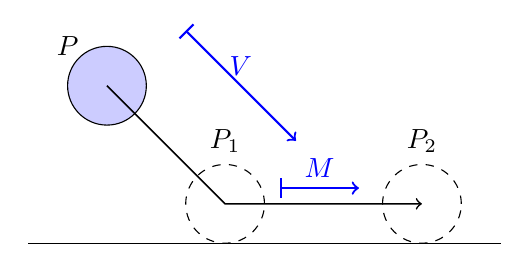
\begin{tikzpicture}
	\draw[fill=blue!20] (1,2) circle (5mm);
	\draw[dashed] (2.5,0.5) circle (5mm) ;
	\draw[dashed] (5,0.5) circle (5mm);
	\draw (0,0) -- (6,0);
	\draw[|->,thick,blue] (2,2.7) -- node[above] {$V$} ++(1.4,-1.4);
    \draw[|->,thick,blue] (3.2,0.7) -- node[above] {$M$} ++(1,0);
	\draw[->,semithick] (1,2) -- (2.5,0.5) -- (5,0.5);
	\draw (0.5,2.5) node {$P$};
	\draw (2.5,1.3) node {$P_1$};
	\draw (5,1.3) node {$P_2$};
\end{tikzpicture}
\caption{Collision and sliding}
\label{fig:collision_sliding}
\end{figure}

\paragraph{Code}
When an actor must be able to collide with its surrounding, some scripting code is required, especially because the engine is unaware of the kind of game the project is part of. For a platform game, the logic is like in Figure \ref{fig:collision_flowchart}.
\begin{figure}
\centering
\scalebox{0.8}{
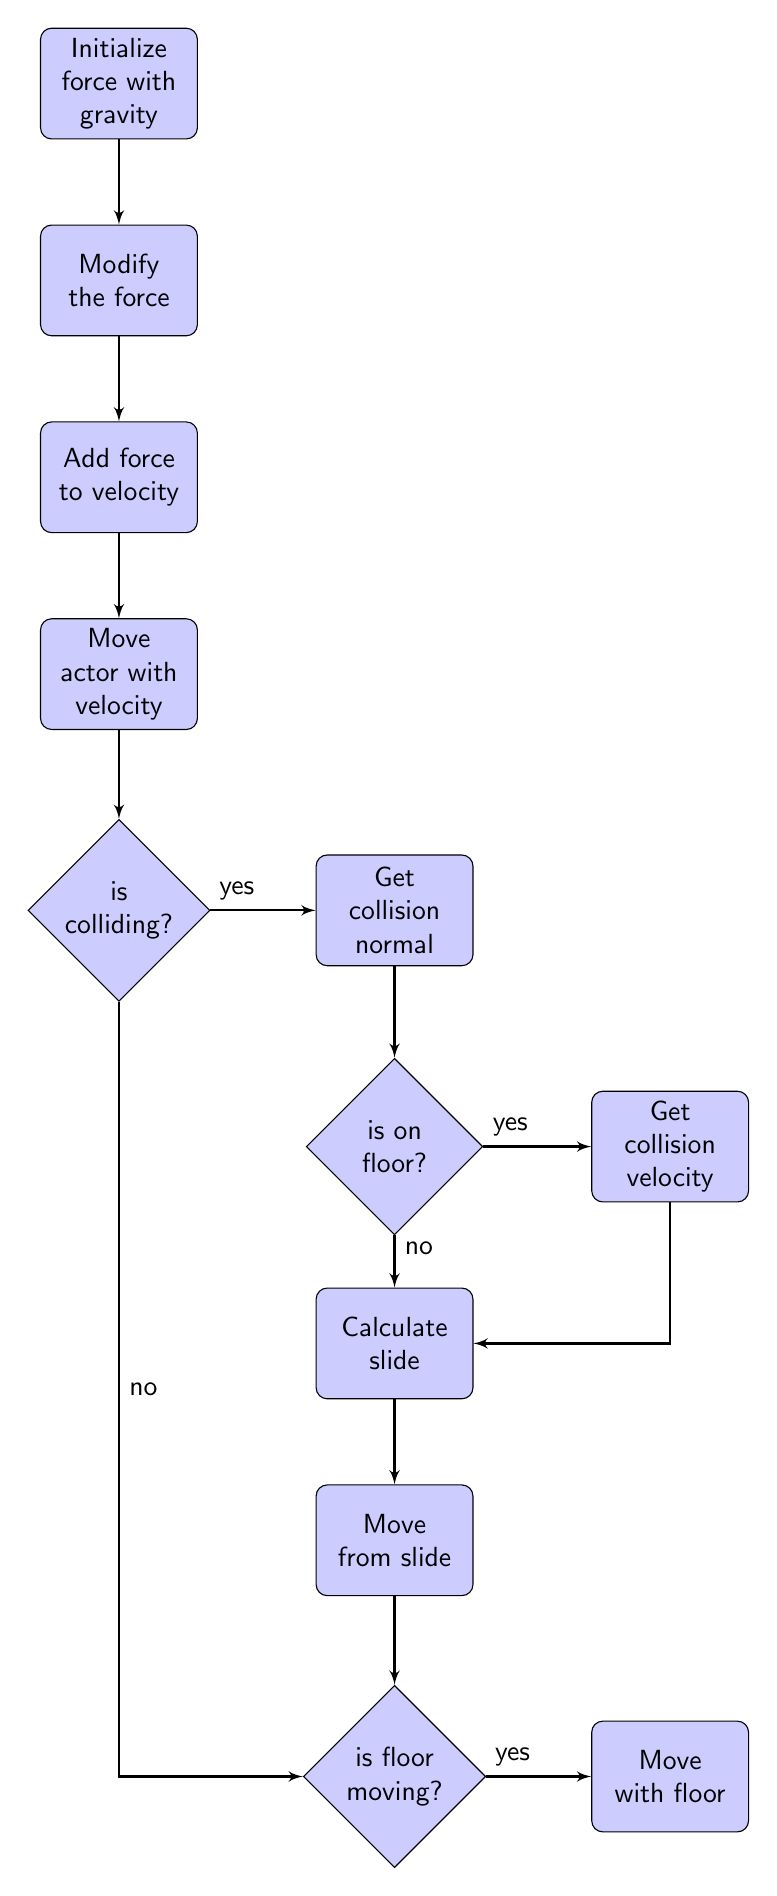
\begin{tikzpicture}[node distance = 2.5cm, auto]
   \node [block] (init) {Initialize force with gravity};
   \node [block,below of=init] (mod_force) {Modify the force};
   \node [block,below of=mod_force] (mod_velocity) {Add force to velocity};   
   \node [block,below of=mod_velocity] (move) {Move actor with velocity};   
   \node [decision,below of=move] (if_collide) {is colliding?};   
   \node [block,right of=if_collide,node distance = 3.5cm] (collision_normal) {Get collision normal};   
   \node [decision,below of=collision_normal] (if_on_floor) {is on floor?};   
   \node [block,right of=if_on_floor,node distance = 3.5cm] (collision_velocity) {Get collision velocity};   
   \node [block,below of=if_on_floor] (slide) {Calculate slide};   
   \node [block,below of=slide] (move_slide) {Move from slide};   
   \node [decision,below of=move_slide] (if_moving_floor) {is floor moving?};   
   \node [block,right of=if_moving_floor,node distance = 3.5cm] (move_floor) {Move with floor};   
   \path [line] (init) -- (mod_force);
   \path [line] (mod_force) -- (mod_velocity);
   \path [line] (mod_velocity) -- (move);
   \path [line] (move) -- (if_collide);
   \path [line] (if_collide) -- node [near start] {yes} (collision_normal);   
   \path [line] (collision_normal) -- (if_on_floor);
   \path [line] (if_on_floor) -- node [near start] {yes} (collision_velocity);   
   \path [line] (collision_velocity) |- (slide);
   \path [line] (if_on_floor) -- node [near start] {no} (slide);   
   \path [line] (if_collide) |- node [near start] {no} (if_moving_floor);   
   \path [line] (slide) -- (move_slide);
   \path [line] (move_slide) -- (if_moving_floor);
   \path [line] (if_moving_floor) -- node [near start] {yes} (move_floor);
\end{tikzpicture}
}
\caption{Collision flowchart}
\label{fig:collision_flowchart}
\end{figure}

\clearpage

\subsection{Traversable platforms}
One issue that comes with using physics in a 2d platform game is the loss of features from older 2d games without physics. One of the most useful ones is the ability to go through a wall or a floor in a certain direction but not the other direction. Typically that would be a floor that the player can jump through from below but not from above. \\
As in Figure \ref{fig:traversable_floor}, actor 1 lands like usual on the box but actor 2 can jump through the box. And once it's above the box, actor 2 cannot go in any more.

\begin{figure}[h]
\centering
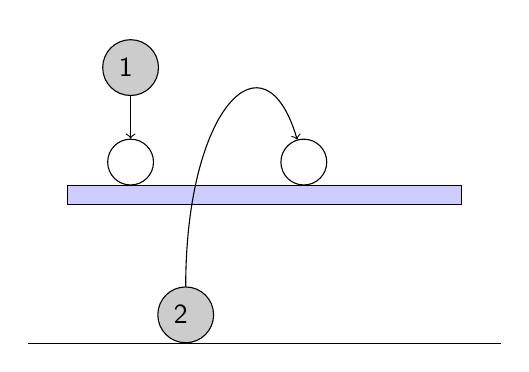
\begin{tikzpicture}
	\draw (0,0) -- (6,0); % floor
	\node[draw,rectangle,fill=blue!20,minimum width=5cm,minimum height=0.2cm] at (3,1.88) {};
	\node[circle,draw=black,fill=black!20,text width=0.3cm] (startPoint) at (2,0.36) {2};
	\node[circle,draw=black,text width=0.3cm] (endPoint) at (3.5,2.3) {};
	\path[->,draw] (startPoint) .. controls (2,3) and (3,4) .. (endPoint);
	\node[circle,draw=black,fill=black!20,text width=0.3cm] (startPoint2) at (1.3,3.5) {1};
	\node[circle,draw=black,text width=0.3cm] (endPoint2) at (1.3,2.3) {};
	\path[->,draw] (startPoint2) -- (endPoint2);
\end{tikzpicture}
\caption{Traversable floor}
\label{fig:traversable_floor}
\end{figure}

\paragraph{Problem}
By default it's impossible to do such thing in Godot. The actor would never be able at any moment to be in the box or any other object. Such state is not allowed by the engine.
It is possible to disable the collision feature of the actor until it got outside of the box, but during this time it would not collide with anything at all. No bonus, no enemy, no bullet, nothing. It would be some kind of unwanted invulnerability that happens every time the actor jump, which is not realistic for a platform game.
\paragraph{Solution}
However, with the collision layers feature, it became possible to disable collision detection of the actor with all objects of a specific layer, just by removing the actor from this layer for the time it needs to go through, usually when its vertical velocity is going up.

\subsection{Vacuum cone \& edible objects}
When the player starts to suck, a vacuum cone is created. Some kind of actors that are within this cone will be sucked to the player's mouth and be eaten. Those actors can be as well enemies, bombs, bonuses or mere blocks. In this demo, they are all extending the abstract class Edible. In a bigger project, it would be better to use duck typing instead and give then a property edible.

\paragraph{Process}
When the player presses the inhale button, the process goes as in Figure \ref{fig:vacuum_process}.
\begin{figure}
\centering
\scalebox{0.9}{
\begin{sequencediagram}
\newthread[white]{p}{Player}
\newinst[2]{c}{Cone}
\newthread{e}{Edible}

\begin{call}{p}{start inhale}{c}{stop inhale}
  \begin{sdblock}{Loop}{}
    \begin{call}{c}{\shortstack{wait for \\edible}}{c}{}
    \end{call}
  \end{sdblock}

  \begin{sdblock}{if edible in area}{}

    \begin{call}{c}{detect}{e}{\shortstack{reachs\\eat\\zone}} 
      \begin{call}{e}{disable behavior}{e}{}
      \end{call}  
      \begin{sdblock}{Loop}{}
        \begin{call}{e}{move to eat zone}{e}{}
        \end{call}
      \end{sdblock}
      \postlevel
    \end{call}

    \begin{messcall}{c}{\shortstack{set charged\\or give bonus}}{p}{}
    \end{messcall}

    \begin{messcall}{c}{absorbe}{e}{}
      \begin{call}{e}{die}{e}{}
      \end{call}  
    \end{messcall}
  \end{sdblock}

  \begin{sdblock}{if timeout and input released}{}
    \begin{messcall}{p}{interrupt}{c}{}
    \end{messcall}
    
    \begin{call}{e}{\shortstack{resume behavior\\after timeout\\if being sucked}}{e}{}
    \end{call}
    
  \end{sdblock}

  \begin{call}{c}{die}{c}{}
  \end{call}  

    
\end{call}
\end{sequencediagram}
}
\caption{Vacuum process}
\label{fig:vacuum_process}
\end{figure}

\paragraph{Node Structure}
Its root is an Area2D.
It is composed of: \\
\begin{tabular}{ l  l }
  \textit{particles} & Particle emitter \\
  \textit{ParticleAttractor2D} & Attractor of the particles \\
  \textit{CollisionPolygon2D} & Vacuum area where Edible objects start to get sucked \\
  \textit{eatPosition} & Position used by Edible objects to know where to be sucked \\
  \textit{eatArea} & Area where sucked objects are considered to be eaten \\
  \textit{sfx} & Sound manager \\
\end{tabular}

\paragraph{Visual effect}
The cone is actually a particular case of particle emitter. Instead of emitting from a point to a direction, it emits in a region to the direction of a single point (see Figure \ref{fig:cone}).

\begin{figure}[h]
\centering
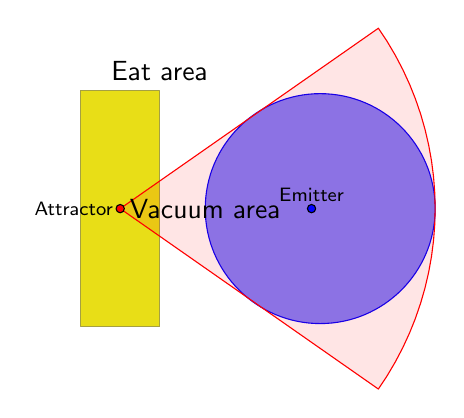
\begin{tikzpicture}[line cap=round,line join=round,>=triangle 45,x=1.0cm,y=1.0cm]
\draw[draw=black!40!yellow,shift={(-0.5,-1.5)},fill=black!10!yellow] rectangle (1,3) node[above] {Eat area};
\draw [color=blue,fill=blue,fill opacity=0.5] (2.54,0) circle (1.46cm);
\draw [draw=red,fill=red,fill opacity=0.1]  (0,0) --  plot[domain=-0.61:0.61,variable=\t]({1*4*cos(\t r)+0*4*sin(\t r)},{0*4*cos(\t r)+1*4*sin(\t r)}) -- cycle node[right,fill opacity=1]{\color{black}Vacuum area};
\begin{scriptsize}
\draw [fill=red] (0,0) circle (1.5pt) node[left] {Attractor};
\draw [fill=blue] (2.43,0) circle (1.5pt) node[above] {Emitter};
\end{scriptsize}
\end{tikzpicture}
\caption{Vacuum cone}
\label{fig:cone}
\end{figure}

\subsection{Scene loading}
Scene loading consist of loading the asset and replace the node of the current scene with this one. The most basic example would be to replace the child of the \textit{/root} node, which then replaces everything visible. In this demo however, there's an HUD and others nodes that need to stay, mosty in order to not add a copy of them in each scene. A special node exists then to contain the currently loaded scene.
\paragraph{Cutscenes and playable scenes}
There are two kinds of scenes. The cutscenes and the playable scenes. The technical difference is that HUD don't show up in cutscenes. But nothing prevents to make a cutscene playable by adding to it a playable character and make the HUD visible again. However the way to load the scene differ from a cutscene to a playable scene. For a cutscene, it's only needed to replace the current scene with the cutscene to load. And for a playable scene, the player, which must have an instance in every playable scene, have to be moved to a certain position determined by a parameter.
\paragraph{Doors}
The parameter defining where the player must be exists because of a need to enter a scene from multiple entry points. A good example is a town with houses. The player start, for instance, at the entrance of the town. And he can visit houses, which are smaller but distinct scenes. That means the player can travel through scenes and go back to the main scene, the town. And in sake of coherence, the player leaving a house should appear at the front of the house instead of the entrance of the town. This problem is solved by passed a parameter to where the player come from.\\
In this demo, doors act like areas where the player travel to another scene. And position nodes with a name are used to determine the new position of the player. The door node has two parameters: the name of the scene to load and the name of the position node to use.
\paragraph{Groups}
The player node doesn't travel through scenes. It is destroyed as the same time as its corresponding scene is destroyed. The player of the new scene is then used to play, making the illusion the player travelled to another scene.\\
The path to the player node is however unknown, as it may not be consistent through scenes. To solve this problem, groups are used. A group is a tag that nodes can have. The player has the tag "Player". It is then possible to retrieve every node of a group. In the case of the player, there is only one node in the group "Player", which makes it easy to find. There is also a group called "entry\_point" which contains all nodes where the player can appear, in order to make easy to find the node by the name given in parameter from the door. 
\paragraph{2 players bug}
There is still a trick with the way scenes are loaded. The code is very simple:
\begin{enumerate}
\item Remove the old scene from the container.
\item Call \textit{queue\_free()} of the old scene to destroy it.
\item Load the new scene.
\item Insert the instance of the new scene in the container.
\item Search the player in the group "Player".
\item Move the found player.
\end{enumerate}
But in point 5, the player of the old scene is still returned, in addition of the player of the new scene. The reason is that the old scene is marked to be freed by the garbage collector but is still existing. And since the array of nodes returned by the search group function is in an unpredictable order, there is no easy way to know which player to move is the good one (from the new scene). This can be easily solved by moving indiscriminately all players, because the old player will be disposed soon anyway and doesn't matter anymore.

\begin{thebibliography}{1}

\bibitem{godot} Godot Game Engine {\em Okam Studio} 2014. 
http://www.godotengine.org/wp/

\bibitem{kirby} Kirby\textcopyright \  is a property of Nintendo\cite{nintendo}.

\bibitem{nintendo} Nintendo Co., Ltd.\textcopyright

\end{thebibliography}

\end{document}
